% !TeX encoding = UTF-8
% !TeX root = ../main.tex

%% ------------------------------------------------------------------------
%% Copyright (C) 2021 SJTUG
%% 
%% SJTUBeamer Example Document by SJTUG
%% 
%% SJTUBeamer Example Document is licensed under a
%% Creative Commons Attribution-NonCommercial-ShareAlike 4.0 International License.
%% 
%% You should have received a copy of the license along with this
%% work. If not, see <http://creativecommons.org/licenses/by-nc-sa/4.0/>.
%% -----------------------------------------------------------------------

\section{Research}

\subsection{Problems}

%\begin{frame}{Research problems}
%\begin{enumerate}
%\item Organizational \textbf{P2P networks} (universities message system): \alert{efficiency?} (messaging time spent and memory space used) $\rightarrow$ \textbf{energy sustainability?}
%\item University network connections (graph theory): \textbf{predicting and recommending partners}: trust? $\rightarrow$ \textbf{links reliability?} \alert{(Machine Learning techniques)}
%\item \textbf{Competitive application calls}: \alert{auction theory (mechanism design)} auditability? $\rightarrow$ \textbf{meritocracy?}
%\end{enumerate}
%\begin{alertblock}{Research studies on practical applications?}
%So far, plenty of theoretical research on blockchain technologies but lack of empirical evidence on real-world practical applications (non-mature and complex technology)
%\end{alertblock}
%\end{frame}

\subsection{The privacy-preserving of Federated Learning}
\begin{frame}{The privacy-preserving of Federated Learning}
    \begin{itemize}
        \item FL provides an attractive structure for decomposing the overall machine learning workflow into the approachable modular units we desire.%(presented in (Kairouz et al.))
        \item FL provides a level of privacy to participating users through data minimization.
    \end{itemize}
    \begin{figure}[h]
        \centering
        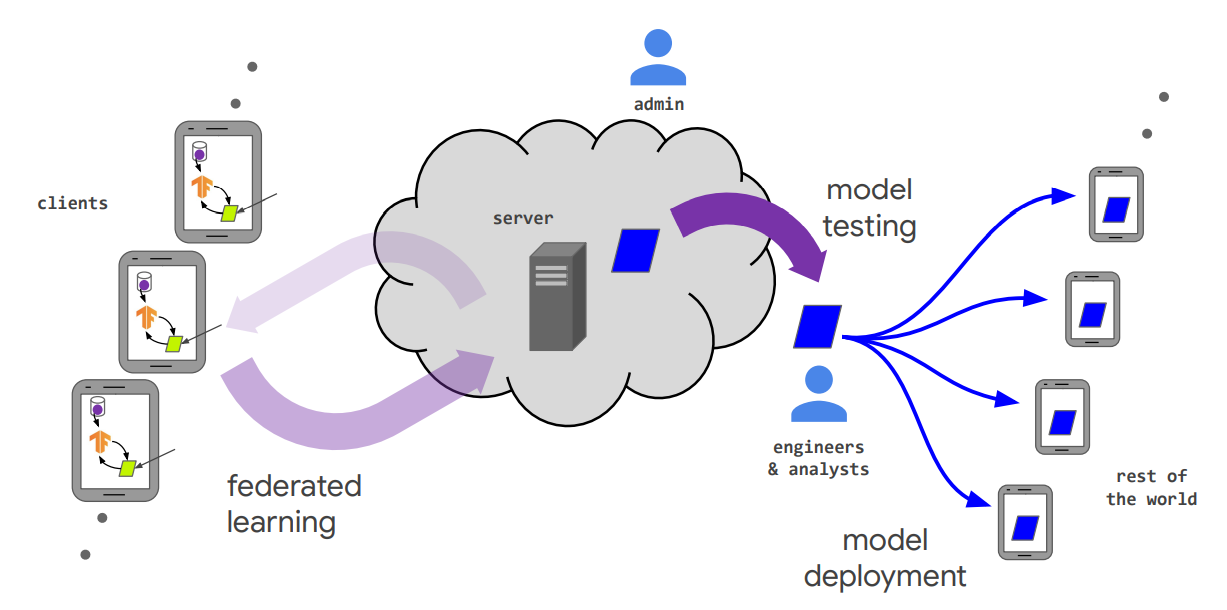
\includegraphics[width=8cm]{structureFL.PNG}
    \end{figure}
\end{frame}

\subsection{The incentive mechanism of Federated Learning}
\begin{frame}{The incentive mechanism of Federated Learning}
  \begin{itemize}
    \item Main types of incentive mechanisms:
          \begin{enumerate}
            \item \alert{Monetary-based}: distributing rewards. %And two subtypes can be considered\cite{paper16}:
            	% \begin{itemize}
            	% \item \alert{price-decision-first} (auction theory) design optimal mechanism benefiting both requesters adn workers
            	% \item \alert{upload-decision-first}: distributing rewards base on the uploaded data (quality)
          		% \end{itemize}
            \item \alert{Reputation-based}: reputation framework for worker selection (algorithms)
          \end{enumerate}
    \item \textbf{Limitations}
    	\begin{enumerate}
            \item Relies on a central platform, vulnerable to target attacks
            \item Single-attribute incentive mechanisms (multifactor incentive needed)
          \end{enumerate}
     %Some previous hybrid incentive mechanisms\cite{paper52} suffer of usability problems because the difficulty of hybrid data management
  \end{itemize}
\end{frame}

%\section{Research}
%
%\subsection{Problems}
%
%\begin{frame}{Blockchain background}
%  \alert{Distributed ledger containing a time-stamped series of immutable blockchains, trustless, decentralized, proof-tampering and full traceability}
%%   \begin{itemize}
%%     \item Research approaches on blockchain-based crowdsensing:
%%           \begin{itemize}
%%             \item Evaluating time consumption and task cost of applying a blockchain-based system\cite{paper33}
%%             \item Blockchain-based crowdsensing quality control model\cite{paper34}
%%             \item Considering privacy issues\cite{paper35}
%%             \item Handling location privacy protection\cite{paper37} (confusion mechanism)
%%           \end{itemize}
%%   \end{itemize}
%    \begin{figure}[h]
%        \centering
%        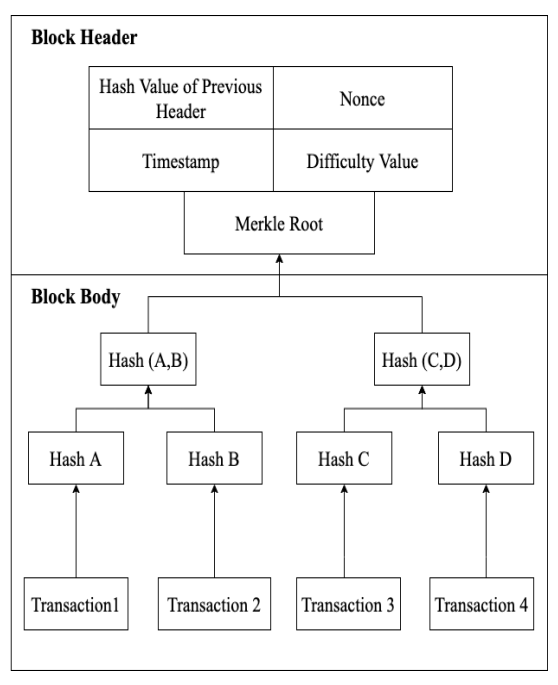
\includegraphics[width=8cm]{topologyBC.PNG}
%    \end{figure}
%\end{frame}
%
%%\begin{frame}{Research problems}
%%\begin{enumerate}
%%\item Organizational \textbf{P2P networks} (universities message system): \alert{efficiency?} (messaging time spent and memory space used) $\rightarrow$ \textbf{energy sustainability?}
%%\item University network connections (graph theory): \textbf{predicting and recommending partners}: trust? $\rightarrow$ \textbf{links reliability?} \alert{(Machine Learning techniques)}
%%\item \textbf{Competitive application calls}: \alert{auction theory (mechanism design)} auditability? $\rightarrow$ \textbf{meritocracy?}
%%\end{enumerate}
%%\begin{alertblock}{Research studies on practical applications?}
%%So far, plenty of theoretical research on blockchain technologies but lack of empirical evidence on real-world practical applications (non-mature and complex technology)
%%\end{alertblock}
%%\end{frame}
%
%\subsection{The privacy-preserving of crowdsensing}
%\begin{frame}{The privacy-preserving of crowdsensing}
%    \begin{itemize}
%        \item FL provides an attractive structure (presented in (Kairouz et al.)) for decomposing the overall machine learning workflow into the approachable modular units we desire.
%        \item FL provides a level of privacy to participating users through data minimization.
%    \end{itemize}
%    \begin{figure}[h]
%        \centering
%        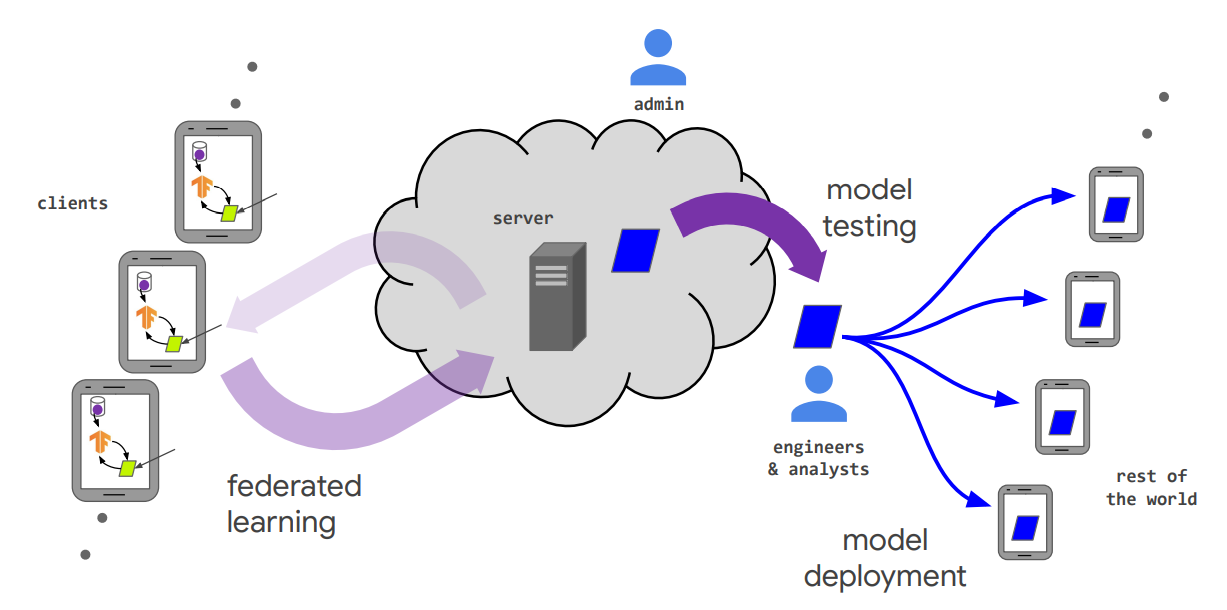
\includegraphics[width=8cm]{structureFL.PNG}
%    \end{figure}
%\end{frame}
%
%\subsection{The incentive mechanism of crowdsensing}
%\begin{frame}{The incentive mechanism of crowdsensing}
%  \begin{itemize}
%    \item Main types of incentive mechanisms:
%          \begin{enumerate}
%            \item \alert{Monetary-based}: distributing rewards. %And two subtypes can be considered\cite{paper16}:
%            	% \begin{itemize}
%            	% \item \alert{price-decision-first} (auction theory) design optimal mechanism benefiting both requesters adn workers
%            	% \item \alert{upload-decision-first}: distributing rewards base on the uploaded data (quality)
%          		% \end{itemize}
%            \item \alert{Reputation-based}: reputation framework for worker selection (algorithms)
%          \end{enumerate}
%    \item \textbf{Limitations}
%    	\begin{enumerate}
%            \item Relies on a central platform, vulnerable to target attacks
%            \item Single-attribute incentive mechanisms (multifactor incentive needed)
%          \end{enumerate}
%     %Some previous hybrid incentive mechanisms\cite{paper52} suffer of usability problems because the difficulty of hybrid data management
%  \end{itemize}
%\end{frame}
%
%%\section{Research}
%%
%%\subsection{Problems}
%%
%%\begin{frame}{Blockchain background}
%%  \alert{Distributed ledger containing a time-stamped series of immutable blockchains, trustless, decentralized, proof-tampering and full traceability}
%%  \begin{itemize}
%%    \item Research approaches on blockchain-based crowdsensing:
%%          \begin{itemize}
%%            \item Evaluating time consumption and task cost of applying a blockchain-based system\cite{paper33}
%%            \item Blockchain-based crowdsensing quality control model\cite{paper34}
%%            \item Considering privacy issues\cite{paper35}
%%            \item Handling location privacy protection\cite{paper37} (confusion mechanism)
%%          \end{itemize}
%%  \end{itemize}
%%\end{frame}
%%
%%%\begin{frame}{Research problems}
%%%\begin{enumerate}
%%%\item Organizational \textbf{P2P networks} (universities message system): \alert{efficiency?} (messaging time spent and memory space used) $\rightarrow$ \textbf{energy sustainability?}
%%%\item University network connections (graph theory): \textbf{predicting and recommending partners}: trust? $\rightarrow$ \textbf{links reliability?} \alert{(Machine Learning techniques)}
%%%\item \textbf{Competitive application calls}: \alert{auction theory (mechanism design)} auditability? $\rightarrow$ \textbf{meritocracy?}
%%%\end{enumerate}
%%%\begin{alertblock}{Research studies on practical applications?}
%%%So far, plenty of theoretical research on blockchain technologies but lack of empirical evidence on real-world practical applications (non-mature and complex technology)
%%%\end{alertblock}
%%%\end{frame}
%%
%%\subsection{The privacy-preserving of crowdsensing}
%%
%%\subsection{The incentive mechanism of crowdsensing}
%%
%%\begin{frame}{The incentive mechanism of crowdsensing}
%%  \begin{itemize}
%%    \item Main types of incentive mechanisms:
%%          \begin{enumerate}
%%            \item \alert{Monetary-based}: distributing rewards. And two subtypes can be considered\cite{paper16}:
%%            	\begin{itemize}
%%            	\item \alert{price-decision-first} (auction theory) design optimal mechanism benefiting both requesters adn workers
%%            	\item \alert{upload-decision-first}: distributing rewards base on the uploaded data (quality)e
%%          		\end{itemize}
%%            \item \alert{Reputation-based}: reputation framework for worker selection (algorithms)
%%          \end{enumerate}
%%    \item \textbf{Limitations}
%%    	\begin{enumerate}
%%            \item Relies on a central platform, vulnerable to target attacks
%%            \item Single-attribute incentive mechanisms (multifactor incentive needed)
%%          \end{enumerate}
%%     Some previous hybrid incentive mechanisms\cite{paper52} suffer of usability problems because the difficulty of hybrid data management
%%  \end{itemize}
%%\end{frame}